\documentclass[11pt]{article}
\usepackage{hyperref}
\usepackage{amsthm}
\usepackage{amsmath}
\usepackage{amsfonts}
\usepackage{tikz}
\usepackage{ wasysym }
\usetikzlibrary{tikzmark}
\usetikzlibrary{arrows.meta}
\usetikzlibrary{shapes}

\newtheorem{example}{Example}


\author{}
\title{}

\begin{document}
%\maketitle
{\Large
%Change Document name to: Graded Homework 1\_Jacob\_Nicholas
\noindent NAME:  Nicholas Jacob\\ 
STUDENT ID: \# 113578513\\
GRADED HOMEWORK NUMBER: 3 Question 3\\
COURSE: CS/DSA 4513 DATABASE MANAGEMENT\\ 
SECTION: ONLINE\\SEMESTER: FALL 2023\\
INSTRUCTOR:  DR. LE GRUENWALD\\
 SCORE:}

\newpage
\begin{enumerate} 
\item First I will consider that the records have freshly been inserted and no reordering on the physical system has been re-done.  This will require pointers going every which way...  The first pointer goes to Black...

\begin{tabular}{|c|c|c|c|c|}\hline
Johnson&11&Yukon&\$20&\tikzmark{jo}\\ \hline
Black&33&OKC&\$20&\tikzmark{bl}\\ \hline
Grant &22&Norman &\$15&\tikzmark{gr}\\ \hline\hline
White&77&OKC&\$20&\tikzmark{wh}\\ \hline
Chapman&44&Edmond&\$20&\tikzmark{ch}\\ \hline
Ford&66&Enid&\$25&\tikzmark{fo}\\ \hline\hline
Haas&99&OKC&\$20&\tikzmark{ha}\\\hline
Hougen&88&Yukon&\$25&\tikzmark{ho}\\\hline
Clinton&55&Tulsa&\$25&\tikzmark{cl}\\\hline\hline
&&&&\tikzmark{end}
\end{tabular} 
  
\begin{tikzpicture}[overlay, remember picture, shorten >=.5pt, shorten <=.5pt, transform canvas={yshift=.25\baselineskip}]
    \draw [->] ({pic cs:bl}) [bend left] to ({pic cs:ch});
        \draw [->] ({pic cs:ch}) [bend left] to ({pic cs:cl});    
        \draw [->] ({pic cs:cl}) [bend left] to ({pic cs:fo});
            \draw [->] ({pic cs:fo}) [bend left] to ({pic cs:gr});
                \draw [->] ({pic cs:gr}) [bend left] to ({pic cs:ha});
                    \draw [->] ({pic cs:ha}) [bend left] to ({pic cs:ho});
                        \draw [->] ({pic cs:ho}) [bend left] to ({pic cs:jo});
                            \draw [->] ({pic cs:jo}) [bend left] to ({pic cs:wh});
                            \draw [-||] ({pic cs:wh}) [bend left] to ({pic cs:end});
                            
  \end{tikzpicture}

I could not find the exact arrow used in notes for the last pointer.  I am terminating by having a null pointer.

So clearly this is the result of all those inserts in a row.  We know that the system will rearrange sequential files periodically so let's do that and have the last file be an insert.

\begin{tabular}{|c|c|c|c|c|}\hline

Black&33&OKC&\$20&\tikzmark{bl1}\\ \hline
Chapman&44&Edmond&\$20&\tikzmark{ch1}\\ \hline
Ford&66&Enid&\$25&\tikzmark{fo1}\\ \hline\hline
Grant &22&Norman &\$15&\tikzmark{gr1}\\ \hline
Haas&99&OKC&\$20&\tikzmark{ha1}\\\hline
Hougen&88&Yukon&\$25&\tikzmark{ho1}\\\hline\hline
Johnson&11&Yukon&\$20&\tikzmark{jo1}\\ \hline
White&77&OKC&\$20&\tikzmark{wh1}\\ \hline
Clinton&55&Tulsa&\$25&\tikzmark{cl1}\\\hline\hline
&&&&\tikzmark{end1}
\end{tabular} 
  
\begin{tikzpicture}[overlay, remember picture, shorten >=.5pt, shorten <=.5pt, transform canvas={yshift=.25\baselineskip}]
    \draw [->] ({pic cs:bl1}) [bend left] to ({pic cs:ch1});
        \draw [->] ({pic cs:ch1}) [bend left] to ({pic cs:cl1});    
        \draw [->] ({pic cs:cl1}) [bend left] to ({pic cs:fo1});
            \draw [->] ({pic cs:fo1}) [bend left] to ({pic cs:gr1});
                \draw [->] ({pic cs:gr1}) [bend left] to ({pic cs:ha1});
                    \draw [->] ({pic cs:ha1}) [bend left] to ({pic cs:ho1});
                        \draw [->] ({pic cs:ho1}) [bend left] to ({pic cs:jo1});
                            \draw [->] ({pic cs:jo1}) [bend left] to ({pic cs:wh1});
                            \draw [-||] ({pic cs:wh1}) [bend left] to ({pic cs:end1});
                            
  \end{tikzpicture}
  
That is somewhat less of a mess...

\item For the second question, I assume the index sequentially by name is full cleaned.

\begin{tabular}{|c|c|} \hline
\$15&\tikzmark{15}\\\hline
\$20 &\tikzmark{20}\\ \hline
\$25& \tikzmark{25}\\ \hline
\end{tabular}
\hspace{1in}
\begin{tabular}{|c|}\hline
\tikzmark{151}\\ \hline\hline
\tikzmark{201}\\\hline
\tikzmark{201c}\\\hline
\tikzmark{201a}\\ \hline\hline
\tikzmark{201b}\\\hline
\tikzmark{201d}\\ \hline\hline
\tikzmark{251}\\\hline
\tikzmark{251a}\\ \hline
\tikzmark{251b}\\ \hline
\end{tabular}
\hspace{1in}
\begin{tabular}{|c|c|c|c|c|}\hline
\tikzmark{20b}Black&33&OKC&\$20&\tikzmark{bl2}\\ \hline
\tikzmark{20c}Chapman&44&Edmond&\$20&\tikzmark{ch2}\\ \hline
\tikzmark{25c}Clinton&55&Tulsa&\$25&\tikzmark{cl2}\\\hline\hline
\tikzmark{25f}Ford&66&Enid&\$25&\tikzmark{fo2}\\ \hline
\tikzmark{15g}Grant &22&Norman &\$15&\tikzmark{gr2}\\ \hline
\tikzmark{20h}Haas&99&OKC&\$20&\tikzmark{ha2}\\\hline\hline
\tikzmark{25h}Hougen&88&Yukon&\$25&\tikzmark{ho2}\\\hline
\tikzmark{20j}Johnson&11&Yukon&\$20&\tikzmark{jo2}\\ \hline
\tikzmark{20w}White&77&OKC&\$20&\tikzmark{wh2}\\ \hline
\hline
&&&&\tikzmark{end2}
\end{tabular} 
  
\begin{tikzpicture}[overlay, remember picture, shorten >=.5pt, shorten <=.5pt, transform canvas={yshift=.25\baselineskip}]
    \draw [->] ({pic cs:bl2}) [bend left] to ({pic cs:ch2});
        \draw [->] ({pic cs:ch2}) [bend left] to ({pic cs:cl2});    
        \draw [->] ({pic cs:cl2}) [bend left] to ({pic cs:fo2});
            \draw [->] ({pic cs:fo2}) [bend left] to ({pic cs:gr2});
                \draw [->] ({pic cs:gr2}) [bend left] to ({pic cs:ha2});
                    \draw [->] ({pic cs:ha2}) [bend left] to ({pic cs:ho2});
                        \draw [->] ({pic cs:ho2}) [bend left] to ({pic cs:jo2});
                            \draw [->] ({pic cs:jo2}) [bend left] to ({pic cs:wh2});
                            \draw [-||] ({pic cs:wh2}) [bend left] to ({pic cs:end2});
\draw [->] ({pic cs:15}) [bend left] to ({pic cs:151});
\draw [->] ({pic cs:20}) [bend left] to ({pic cs:201});
\draw [->] ({pic cs:25}) [bend left] to ({pic cs:251});
\draw [->] ({pic cs:201a}) [bend left] to ({pic cs:201b});
\draw [->] ({pic cs:151}) [bend left] to ({pic cs:15g});
      \draw [->] ({pic cs:201}) [bend left] to ({pic cs:20b});     
\draw [->] ({pic cs:201c}) [bend left] to ({pic cs:20c});      
\draw [->] ({pic cs:201a}) [bend left] to ({pic cs:20h});     
\draw [->] ({pic cs:201b}) [bend left] to ({pic cs:20j});           
\draw [->] ({pic cs:201d}) [bend left] to ({pic cs:20w});            
\draw [->] ({pic cs:251}) [bend left] to ({pic cs:25c});              
\draw [->] ({pic cs:251a}) [bend left] to ({pic cs:25f});             
\draw [->] ({pic cs:251b}) [bend left] to ({pic cs:25h});  
  \end{tikzpicture}

So not a terrible mess (although you should see the \LaTeX\ code it took to generate this...)  Highlights include pointers from each dollar amount into sequentially stored pointer of the data (I even kept the three requirement on the \$20 breaking that into two blocks)
\item For creating the B tree of order 3, we will have three pointers to next part of tree available at each block and room for two indexes.  I will follow the algorithm outlined in the notes.
\begin{itemize}
\item First two insertions are trivial.  Just filling the root. $[11,33]$.  
\item As 22 is inserted, we have filled the first block so we get 22 as the root and both 11 and 33 end up in their own blocks.  
\item 77 joins 33.  No issues
\item 44 Will fill that block though so 44 will need to go to the parent.  Let's make that picture!

\begin{tikzpicture}
\tikzstyle{bplus}=[rectangle split, rectangle split horizontal,rectangle split ignore empty parts,draw]
\tikzstyle{every node}=[bplus]
\tikzstyle{level 1}=[sibling distance=60mm]
%\tikzstyle{level 2}=[sibling distance=15mm]
\node {22 \nodepart{two} 44} [->]
  child {node {11}}    
  child {node {33}}    
  child{node {77}};      
\end{tikzpicture}
\item 66 will have a spot but 99 fills that node so 77 will go to the root which fills the root too.  This must split again.  44 is the middle value it becomes the root.  Another picture is in order.
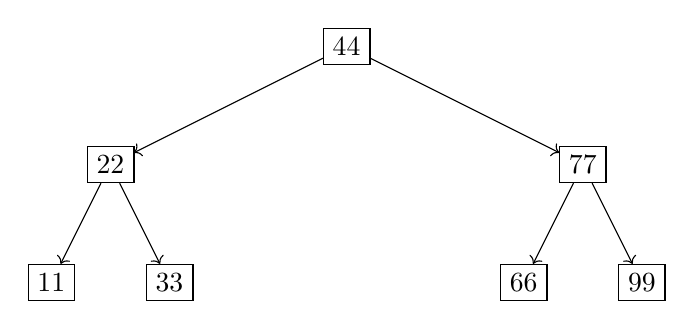
\begin{tikzpicture}
\tikzstyle{bplus}=[rectangle split, rectangle split horizontal,rectangle split ignore empty parts,draw]
\tikzstyle{every node}=[bplus]
\tikzstyle{level 1}=[sibling distance=60mm]
\tikzstyle{level 2}=[sibling distance=15mm]
\node {44} [->]
  child {node {22}
	child {node{11}}
	child {node {33}}
}    
  child {node {77}
	child {node{66}}
	child {node {99}}};      
\end{tikzpicture}
\item 88 and 55 have slots in the leaves.

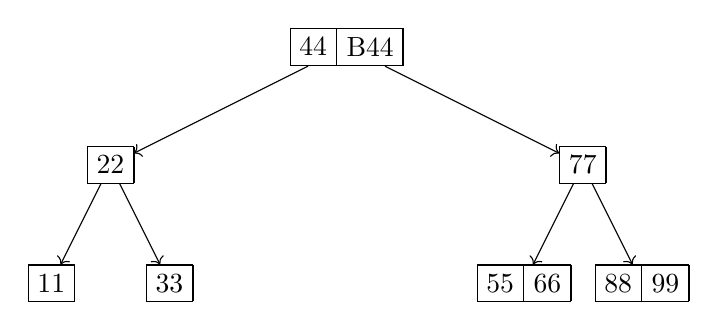
\begin{tikzpicture}
\tikzstyle{bplus}=[rectangle split, rectangle split horizontal,rectangle split ignore empty parts,draw]
\tikzstyle{every node}=[bplus]
\tikzstyle{level 1}=[sibling distance=60mm]
\tikzstyle{level 2}=[sibling distance=15mm]
\node {44\nodepart{two}B44} [->]
  child {node {22}
	child {node{11}}
	child {node {33}}
}    
  child {node {77}
	child {node{55\nodepart{two}66}}
	child {node {88 \nodepart{two}99}}};      
\end{tikzpicture}

\end{itemize}
\end{enumerate}






\end{document}